
\section{Experimental Evaluation and Analysis}
\label{sec:exp}

In this section, we present experimental results to answer the following research questions:

\begin{enumerate}[label=\textbf{(RQ\arabic*)},ref=(RQ\arabic*),leftmargin=*]
    \item\label{RQ1}\gdef\Giref{\ref{RQ1}} How fast is query optimization using meta-decompositions?
	\item\label{RQ2}\gdef\Giref{\ref{RQ2}} How good are width-1 query plans, compared to the globally optimal ones?
    \item\label{RQ3}\gdef\Giref{\ref{RQ3}} To what extent is our proposed meta-decompositions-based query optimization sensitive to errors in cardinality estimation?
    \item\label{RQ4}\gdef\Giref{\ref{RQ4}} To what extent can our proposed meta-decompositions-based join tree enumeration technique help structure-based query evaluation?
\end{enumerate}

\subsection{Experimental Setup}
\subsubsection{Experimental Environment} Experiments are conducted on an Apple M4 Pro machine with 14 cores and 48 GB RAM, running macOS Tahoe 16.0. We use DuckDB as our test database because of its excellent performance and simple cost model. The experiments use DuckDB 1.2.2, Scala 3.6.3, GraalVM 17.0.12, and LLVM 20.1.3. The full source code for experiments is available at~\cite{github}.

We implement \sys{} in Scala. For each query, it first computes the meta-decomposition (Section~\ref{sec:meta}) and then applies our cost-based optimization algorithm (Section~\ref{sec:opt}) to select the best width-1 query plan.  
In the experiments, we compare the following query optimization approaches:
\begin{enumerate}[leftmargin=*]
    \item \sys{}, using our implementation.
    \item DPconv~\cite{stoian_dpconv_2024}, the state-of-the-art dynamic programming optimizer.
    \item DuckDB's native optimizer~\cite{raasveldt_duckdb_2019}, which uses \textsf{DPccp}~\cite{moerkotte_dynamic_2008} for queries with up to 12 relations and Greedy Operator Ordering~(GOO)~\cite{fegaras_new_1998} otherwise.
    \item UnionDP, a heuristic approach proposed in~\cite[Algorithm~4]{mancini_efficient_2022} which (i) partitions the query graph into subgraphs, each with size up to a threshold (which we set to 12, consistent with DuckDB), (ii) runs dynamic programming on each subgraph, and (iii) runs dynamic programming on the entire graph, treating each subgraph as a composite node.
    \item Yannakakis$^+$~\cite{wang_yannakakis_2025}, a state-of-the-art structure-guided query evaluation approach.
    \item LearnedRewrite~\cite{zhou_learned_2023,zhou_learned_2021}, a machine learning--based query rewriter.
    \item LLM-R$^2$~\cite{li_llm-r2_2024}, a query rewriter based on machine learning and large language models (LLMs).
\end{enumerate}
For Yannakakis$^+$, we use the implemented system as a black box and run the rewritten queries in DuckDB.
For LearnedRewrite and LLM-R$^2$, we similarly evaluate them using their pre-trained models as-is and run the rewritten queries in DuckDB.
For \sys{}, DPconv, and UnionDP, the query plans are enforced in DuckDB by rewriting queries into a sequence of subqueries that create a temporary view at each step, as is standard in, e.g., \cite{wang_yannakakis_2025,gottlob_reaching_2023}.  For all three methods, we apply the same strategies of selection and projection pushdown as explained in \cref{sec:prelim-plans}. Namely, we project out all irrelevant attributes (those that are neither in the output nor in subsequent joins) at every step, and we integrate each selection (filter) condition in the join or scan operation at the lowest possible level, i.e., as soon as all relevant attributes exist.

Each query plan is executed $10$ times, and we report the median optimization and execution time. To ensure accuracy, we exclude I/O time from time measurements. The full dataset is preloaded into the DuckDB database, and the estimated cardinalities are preloaded into memory, with all loading time excluded from timing. We enforce a 5-minute timeout on execution time. Queries that none of the optimizers can complete within this time limit are excluded from the results.

\subsubsection{Queries, Benchmarks, and Cardinalities.} We experiment with the following four benchmarks:
\begin{enumerate}[leftmargin=*]
    \item The SPJ (select-project-join) queries in the \textbf{Decision Support Benchmark (DSB)}~\cite{ding_dsb_2021}. We use the implemented system to generate a 10 GB database instance and generate queries using the default settings. We only consider acyclic queries (240 out of 300). 
    \item The \textbf{Join Order Benchmark (JOB)}~\cite{leis_query_2018} over the IMDB dataset. All queries in this benchmark are already acyclic.
    \item \textbf{Musicbrainz}, a benchmark proposed by \cite{mancini_efficient_2022} with significantly larger queries that join up to 26 relations. We use the implemented query generator with default settings, except that we project the output to at most 5 randomly-selected attributes. We retain only the acyclic queries (243 out of 375).
    \item \textbf{JOBLarge}, a new benchmark we introduce to extend JOB to simulate practical but larger analytical scenarios, where each query is generated by selecting two queries from the JOB that share at least one common output attribute and merging them into a single query, with a join on a shared attribute, such that the query remains acyclic. 
% The rationale is to simulate cases where analysts or automated systems often combine independent analytical queries into one larger query to gain deeper insights.
We only retain generated queries that take DuckDB at least 50 ms to evaluate.
\end{enumerate}
In \cref{tab:query-props}, we show detailed statistics of some structural properties of queries in each benchmark.


\begin{footnotesize}
\begin{table}
    \centering
    \begin{tabular}{cc|c|c|c|c|c}
        \hline
        \multicolumn{2}{r|}{\bf{Benchmarks $\rightarrow$}}               & \bf{DSB} & \bf{JOB} & \bf\makecell{Musicbrainz} & \bf\makecell{JOBLarge} & \bf\makecell{Overall} \\ \hline
        \multirow{3}{*}{\bf\shortstack{Number of\\relations}}  & Min     & 5        & 4        & 2                            & 8                         & 2 \\
                                                               & Median  & 6        & 8        & 10                           & 18                        & 8 \\
                                                               & Max     & 9        & 17       & 26                           & 34                        & 34 \\ \hline
        \multirow{3}{*}{\bf\shortstack{Fan-out}}               & Min     & 2        & 2        & 1                            & 2                         & 1 \\
                                                               & Median  & 3        & 3        & 4                            & 4                         & 3 \\
                                                               & Max     & 4        & 5        & 9                            & 5                         & 9 \\ \hline
        \multirow{3}{*}{\bf\shortstack{Number of\\join trees}} & Min     & 5        & 12       & 2                            & 72                        & 2 \\
                                                               & Median  & 7        & 144      & 22500                        & 40000                     & 126 \\
                                                               & Max     & 54       & 352512   & $> 10^8$                     & $> 10^8$                  & $> 10^8$ \\ \hline
    \end{tabular}
    % \vspace{-0.2em}
    \caption
    % of{table}
    {Structural properties of queries in each benchmark}
    \vspace{-1\baselineskip}
    \label{tab:query-props}
\end{table}
\end{footnotesize}


For \sys{}, DPconv, and UnionDP, which all follow the same cost model, we precompute (by running appropriate \texttt{COUNT(*)} queries) true cardinalities of all possible intermediate join results for the relatively small benchmarks DSB and JOB, in the approach and format consistent with the implementation of DPconv~\cite{stoian_dpconv_2024}. 
For the larger benchmarks Musicbrainz and JOBLarge, computing exact cardinalities for all possible intermediate joins is infeasible due to the much larger query sizes. Therefore, we use estimated cardinalities instead, via DuckDB's \texttt{EXPLAIN} command. Note, however, that these estimates may sometimes be highly inaccurate and may not reflect the true relative sizes of intermediate results.
DuckDB, Yannakakis$^+$, Learned Rewrite, and LLM-R$^2$ are used as black boxes with their own cost models.

\subsection{Results}



In this section, we present the results of our experiments.

\subsubsection{\ref{RQ1} Optimization Time}

\begin{figure}
    
\includegraphics[width=\linewidth]{figs/exp/opt-time/opt-time-legend.pdf}
    
    \vspace{0.5\baselineskip}
    
    \begin{subfigure}[b]{0.49\textwidth}
        \centering
        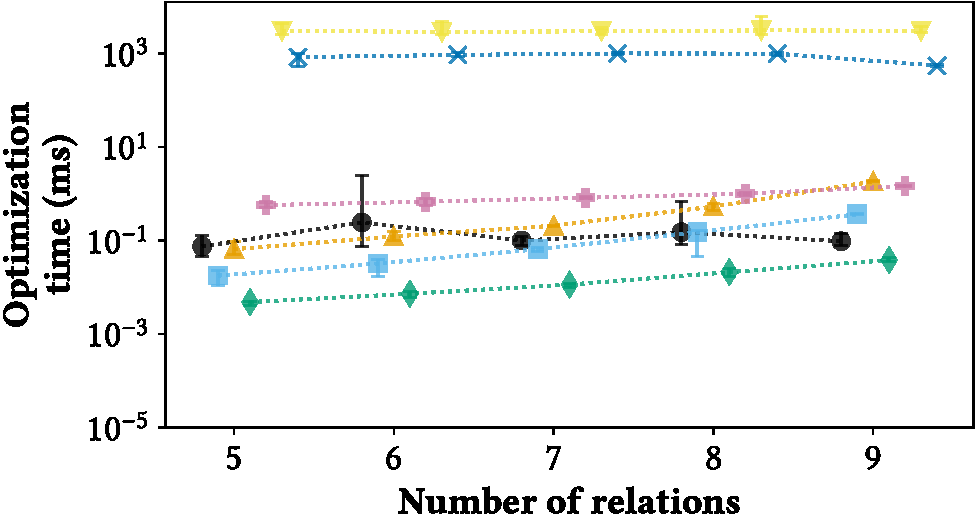
\includegraphics[width=\linewidth]{figs/exp/opt-time/opt-time-dsb.pdf}
        \vspace{-1.25\baselineskip}
        \caption{DSB}
        \label{fig:opt-time-dsb}
    \end{subfigure}
    \hfill
    \begin{subfigure}[b]{0.49\textwidth}
        \centering
        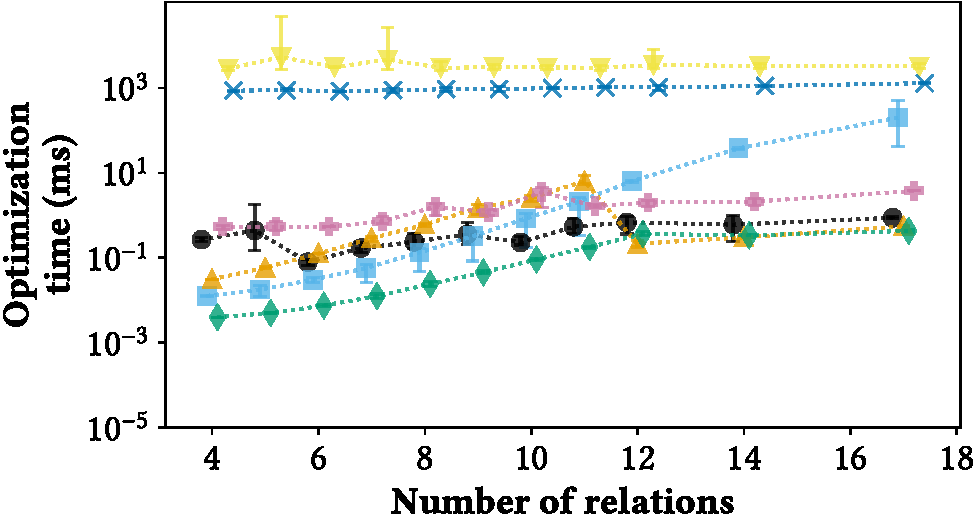
\includegraphics[width=\linewidth]{figs/exp/opt-time/opt-time-job-original.pdf}
        \vspace{-1.25\baselineskip}
        \caption{JOB}
        \label{fig:opt-time-job-original}
    \end{subfigure}
    
    \vspace{0.75\baselineskip}
    
    \begin{subfigure}[b]{0.49\textwidth}
        \centering
        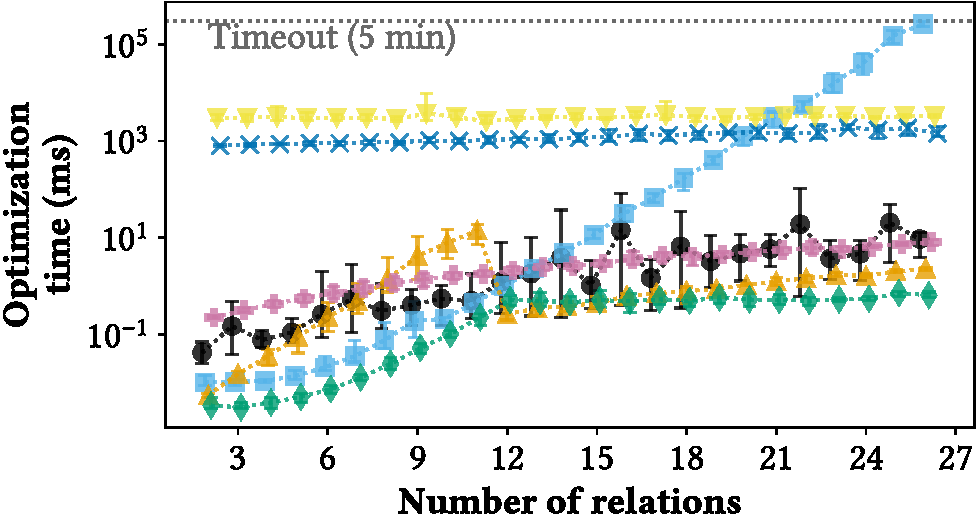
\includegraphics[width=\linewidth]{figs/exp/opt-time/opt-time-musicbrainz.pdf}
        \vspace{-1.25\baselineskip}
        \caption{Musicbrainz}
        \label{fig:opt-time-musicbrainz}
    \end{subfigure}
    \hfill
    \begin{subfigure}[b]{0.49\textwidth}
        \centering
        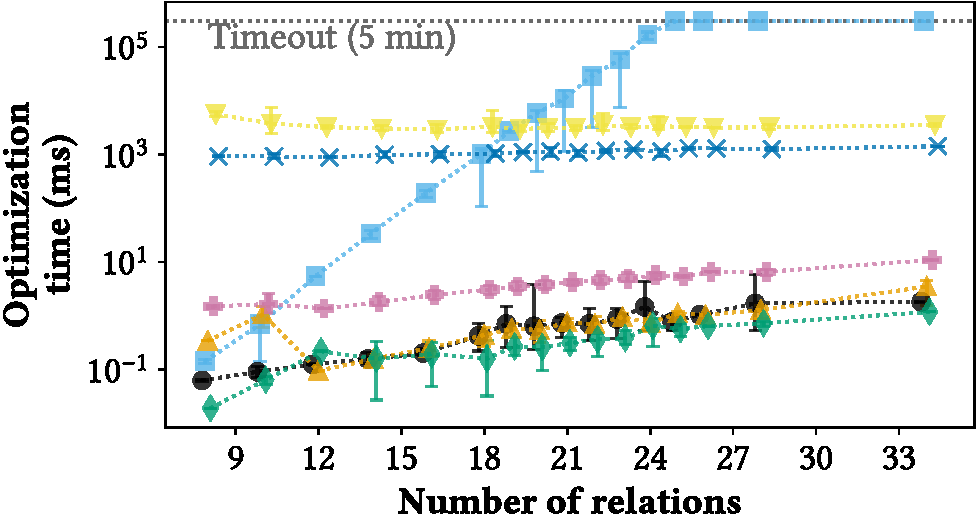
\includegraphics[width=\linewidth]{figs/exp/opt-time/opt-time-job-large.pdf}
        \vspace{-1.25\baselineskip}
        \caption{JOBLarge}
        \label{fig:opt-time-job-large}
    \end{subfigure}
    \vspace{-0.25\baselineskip}
    \caption{Optimization time for queries in each benchmark. For each number of relations, the dot shows the average, and the whiskers show the minimum and maximum optimization time.}
    \label{fig:opt-time-overall}
\end{figure}

We first compare the optimization time. The results are shown in \cref{fig:opt-time-overall}.
The figures clearly show that the optimization time of \sys{} remains almost constant as the number of relations increases, typically below 10 ms, as is also the case for DuckDB, UnionDP, and Yannakakis$^+$.
The two machine learning--based approaches, LLM-R$^2$ and LearnedRewrite, exhibit stable but higher optimization time, in the order of seconds, due to the overhead of the complex models and, for LLM-R$^2$, the interaction with LLMs.
DPconv, however, has an exponential growth, and its optimization time surpasses that of \sys{} starting at approximately 9 relations. 
For many queries in Musicbrainz and JOBLarge (starting from approximately 25 relations), DPconv fails to find a valid plan within the 5-minute limit, again highlighting that traditional exponential-time dynamic programming–based optimizers do not scale to such large queries.

\subsubsection{\ref{RQ2} Quality of width-1 query plans}

Even though \sys{} restricts its search to width-1 plans only, as shown in \cref{fig:cost-ratio}, for most queries, it \emph{finds query plans with cost values comparable to those of the optimal plans}.
Furthermore, \cref{fig:exec-speedup} shows the speedups achieved by executing the optimal width-1 query plans over executing the globally optimal query plans. Note that, even though one would typically not expect speedups since the optimal plans have the minimum possible cost values, in many cases, the optimal width-1 query plans in fact run faster in the actual execution, thanks to the small intermediate result sizes through exploiting queries' structural properties.

% \afterpage{
\begin{figure}
    \begin{subfigure}[b]{0.24\textwidth}
        \centering
        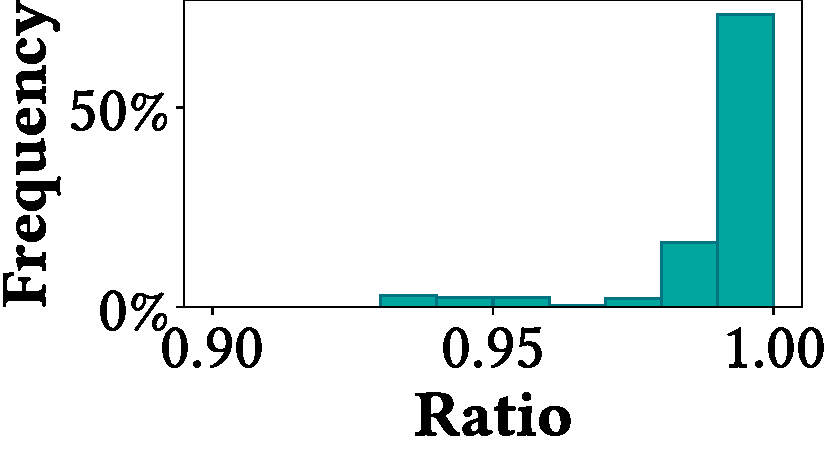
\includegraphics[width=\linewidth]{figs/exp/cost-ratio/cost-ratios-dsb.pdf}
        \vspace{-1.25\baselineskip}
        \caption{DSB}
        \label{fig:cost-ratios-dsb}
    \end{subfigure}
    \hfill
    \begin{subfigure}[b]{0.24\textwidth}
        \centering
        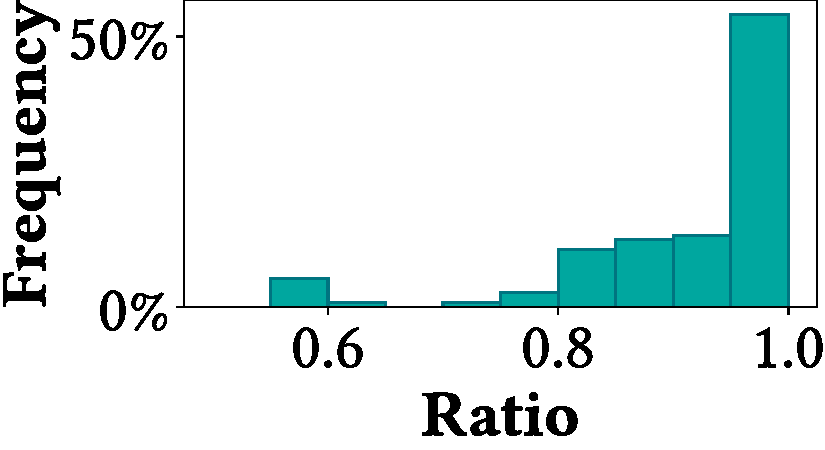
\includegraphics[width=\linewidth]{figs/exp/cost-ratio/cost-ratios-job-original.pdf}
        \vspace{-1.25\baselineskip}
        \caption{JOB}
        \label{fig:cost-ratios-job-original}
    \end{subfigure}
    \hfill
    \begin{subfigure}[b]{0.24\textwidth}
        \centering
        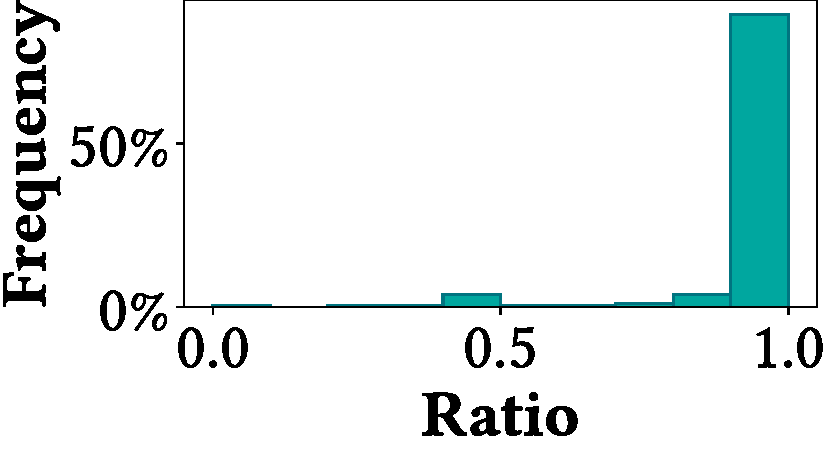
\includegraphics[width=\linewidth]{figs/exp/cost-ratio/cost-ratios-musicbrainz.pdf}
        \vspace{-1.25\baselineskip}
        \caption{Musicbrainz}
        \label{fig:cost-ratios-musicbrainz}
    \end{subfigure}
    \hfill
    \begin{subfigure}[b]{0.24\textwidth}
        \centering
        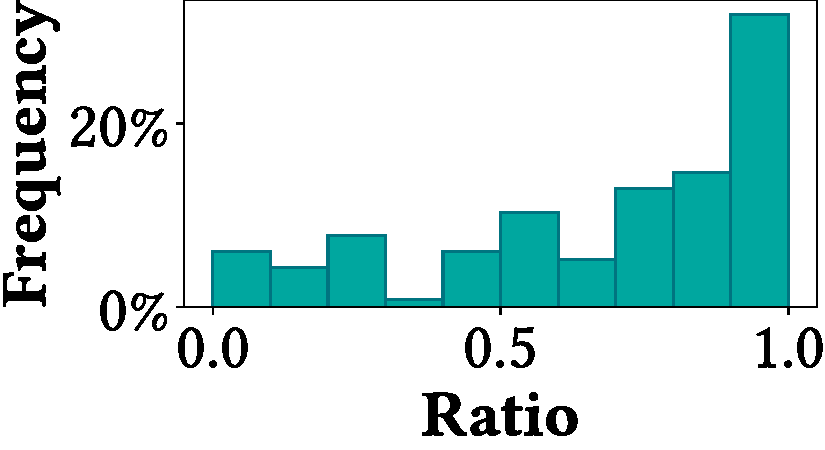
\includegraphics[width=\linewidth]{figs/exp/cost-ratio/cost-ratios-job-large.pdf}
        \vspace{-1.25\baselineskip}
        \caption{JOBLarge}
        \label{fig:cost-ratios-job-large}
    \end{subfigure}
    
    \vspace{-0.5\baselineskip}
    \caption[Ratios between the costs of the globally optimal query plans and the costs of the optimal width-1 plans for queries in each benchmark]{Ratios between the costs of the globally optimal query plans and the costs of the optimal width-1 plans. A ratio of 1 indicates they have the same cost, and is included in the bar between 0.9 and 1.0.\footnotemark[3]}
    \vspace{0.5\baselineskip}
    \label{fig:cost-ratio}
\end{figure}

    \footnotetext[3]{This measure is analogous to speedups. Since width-1 plans are a restricted class, their theoretical cost values cannot be better (lower) than the global optimal, and thus the ratios are at most 1.}

\begin{figure}
    \begin{subfigure}[b]{0.49\textwidth}
        \centering
        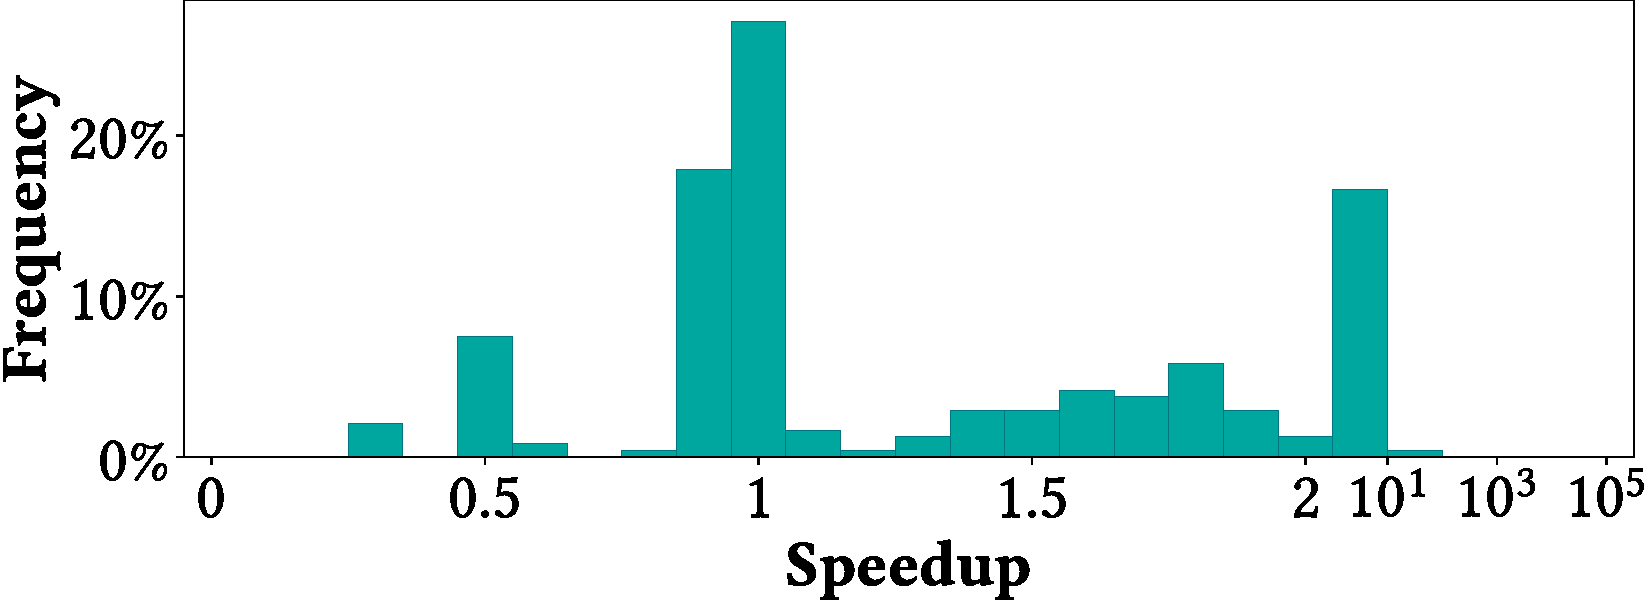
\includegraphics[width=\linewidth]{figs/exp/exec-speedup/exec-speedups-over-dpconv-dsb.pdf}
        \vspace{-1.25\baselineskip}
        \caption{DSB}
        \label{fig:exec-speedup-dsb}
    \end{subfigure}
    \hfill
    \begin{subfigure}[b]{0.49\textwidth}
        \centering
        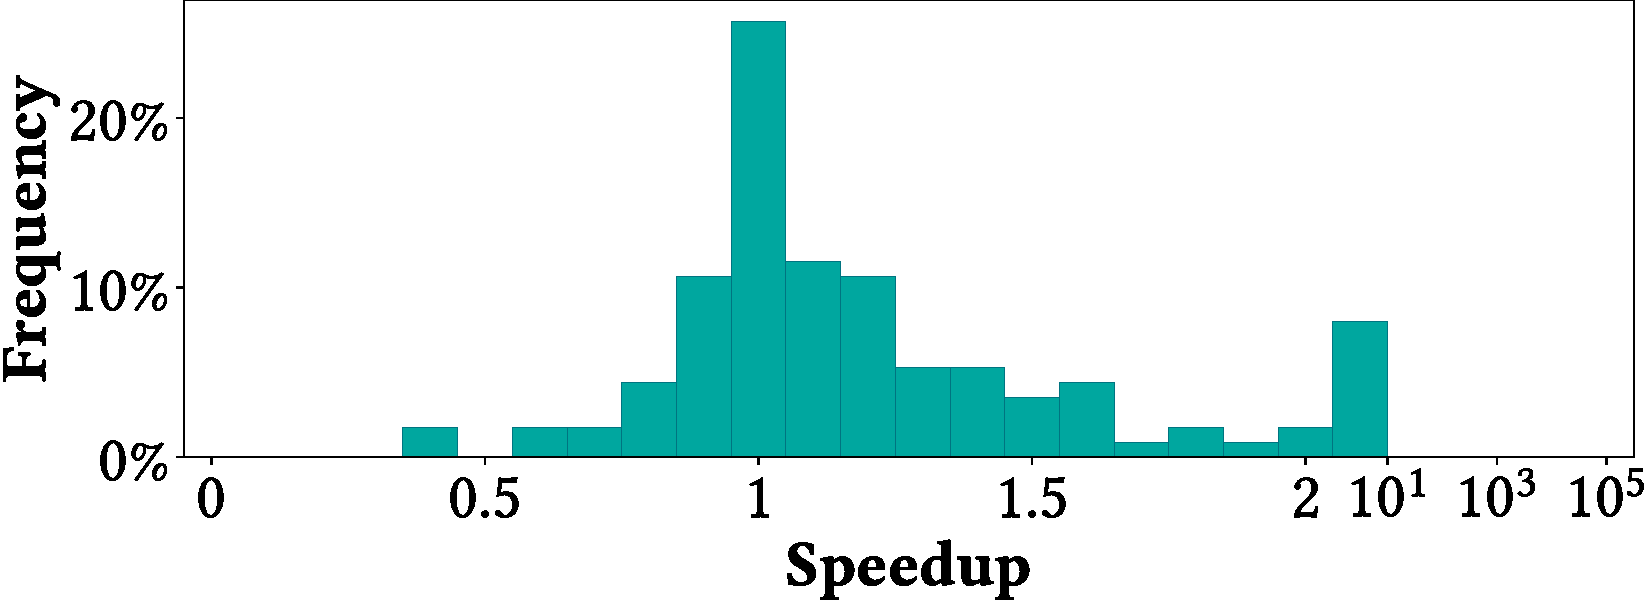
\includegraphics[width=\linewidth]{figs/exp/exec-speedup/exec-speedups-over-dpconv-job-original.pdf}
        \vspace{-1.25\baselineskip}
        \caption{JOB}
        \label{fig:exec-speedup-job-original}
    \end{subfigure}

    \vspace{0.5\baselineskip}

    \begin{subfigure}[b]{0.49\textwidth}
        \centering
        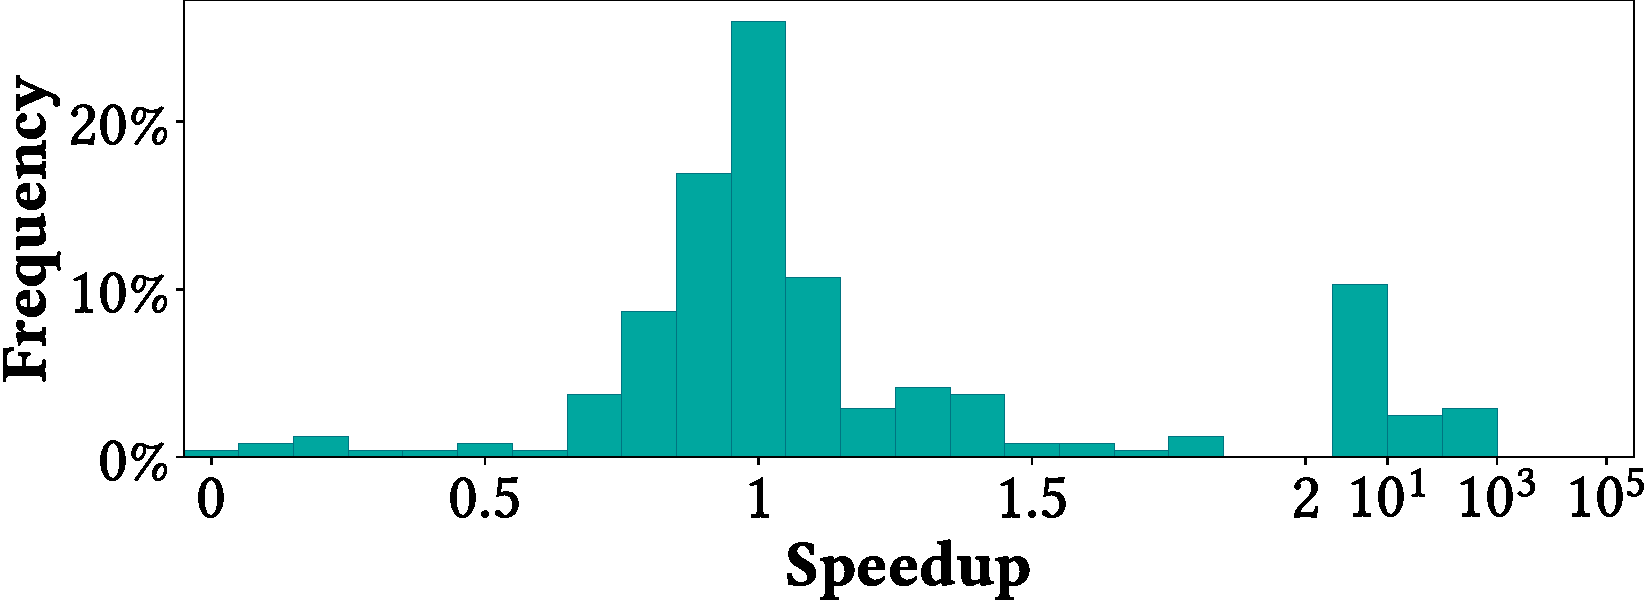
\includegraphics[width=\linewidth]{figs/exp/exec-speedup/exec-speedups-over-dpconv-musicbrainz.pdf}
        \vspace{-1.25\baselineskip}
        \caption{Musicbrainz}
        \label{fig:exec-speedup-musicbrainz}
    \end{subfigure}
    \hfill
    \begin{subfigure}[b]{0.49\textwidth}
        \centering
        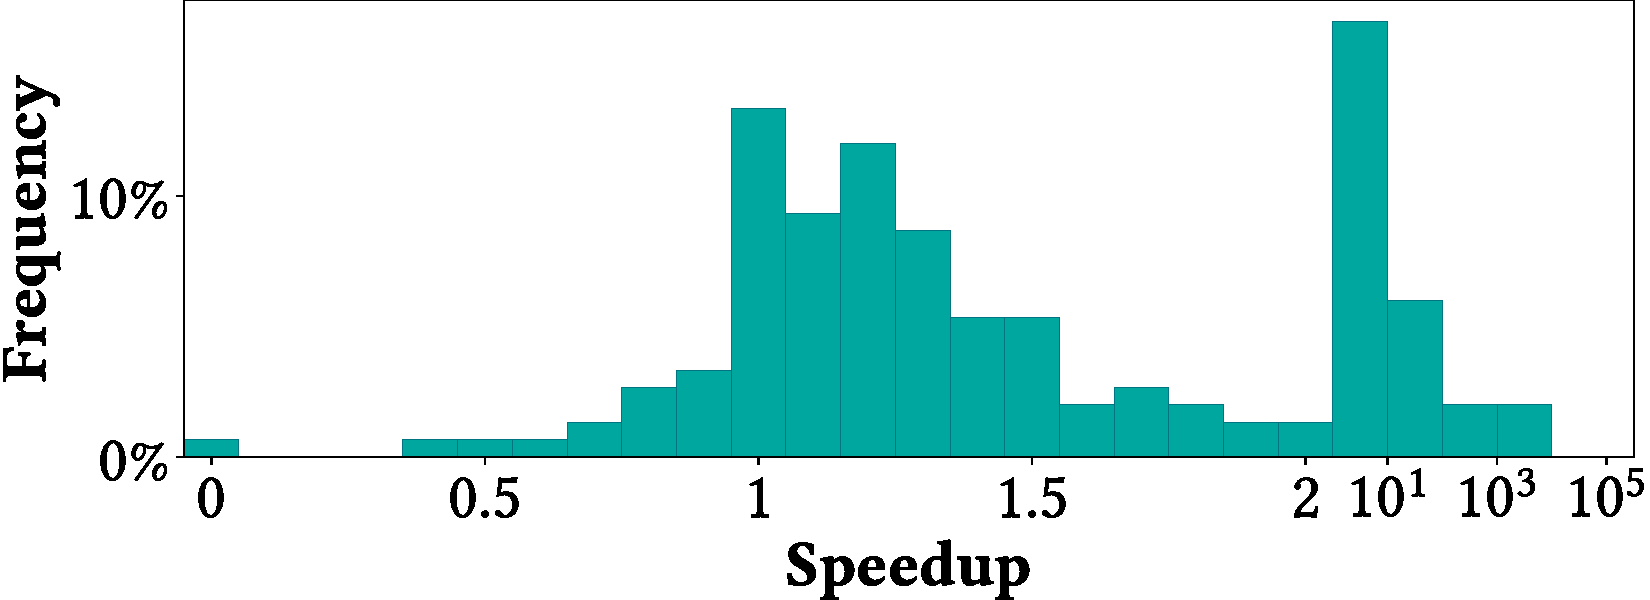
\includegraphics[width=\linewidth]{figs/exp/exec-speedup/exec-speedups-over-dpconv-job-large.pdf}
        \vspace{-1.25\baselineskip}
        \caption{JOBLarge}
        \label{fig:exec-speedup-job-large}
    \end{subfigure}
    
    \vspace{-0.5\baselineskip}
    \caption{Histograms of execution speedups of the optimal width-1 plans over the globally optimal plans}
    \label{fig:exec-speedup}
\end{figure}
% }

\subsubsection{\ref{RQ1} \& \ref{RQ2} Combined: Overall Performance}


% \afterpage{%
    % \clearpage% Flush earlier floats (otherwise order might not be correct)
    % \thispagestyle{empty}% empty page style (?)
    % \begin{landscape}% Landscape page
    % \centering
\begin{table}
    \begin{tiny}
        \renewcommand{\arraystretch}{1.1}
        \setlength\tabcolsep{0.3pt}
        
\begin{tabular}{cr|rrrr|rrrr|rrrr|rrrr}
    \hline
    \multicolumn{2}{r|}{\textbf{Benchmark $\rightarrow$}}
        & \multicolumn{4}{c|}{\textbf{DSB}} & \multicolumn{4}{c|}{\textbf{JOB}} & \multicolumn{4}{c|}{\textbf{Musicbrainz}} & \multicolumn{4}{c}{\textbf{JOBLarge}} \\
    \textbf{Metric $\downarrow$} & \textbf{Method $\downarrow$}
        & Mean & Med. & 95th & 99th & Mean & Med. & 95th & 99th & Mean & Med. & 95th & 99th & Mean & Med. & 95th & 99th \\
    \hline
    \multirow{7}{*}{\bf\rotatebox[origin=c]{90}{Optimization time}}
        & \sys{}  & 0.15 ms & 0.10 ms & 0.32 ms & 1.01 ms & 0.38 ms & 0.26 ms & 0.94 ms & 1.04 ms & 2.62 ms & 0.37 ms & 10.45 ms & 45.05 ms & 0.59 ms & 0.37 ms & 1.67 ms & 4.17 ms \\
        & DPconv  & 0.08 ms & 0.03 ms & 0.36 ms & 0.37 ms & 8.32 ms & 0.16 ms & 38.22 ms & 45.08 ms & 7.37 s & 0.30 ms & 14.62 s & 244.44 s & 42.17 s & 1.26 s & $>$ 5 min & $>$ 5 min \\
        & DuckDB  & 0.32 ms & 0.12 ms & 1.83 ms & 1.87 ms & 1.13 ms & 0.32 ms & 5.58 ms & 8.43 ms & 1.89 ms & 0.47 ms & 11.34 ms & 18.59 ms & 0.62 ms & 0.55 ms & 1.23 ms & 3.81 ms \\
        & UnionDP  & 0.01 ms & 0.007 ms & 0.04 ms & 0.04 ms & 0.10 ms & 0.03 ms & 0.38 ms & 0.45 ms & 0.25 ms & 0.11 ms & 0.64 ms & 0.77 ms & 0.29 ms & 0.24 ms & 0.77 ms & 1.18 ms \\
        & Yannakakis$^+$  & 0.78 ms & 0.70 ms & 1.48 ms & 1.50 ms & 1.44 ms & 1.37 ms & 3.78 ms & 4.59 ms & 2.29 ms & 1.72 ms & 6.43 ms & 8.15 ms & 3.55 ms & 3.27 ms & 6.53 ms & 10.89 ms \\
        & LearnedRew.  & 0.89 s & 0.95 s & 1.03 s & 1.06 s & 0.96 s & 0.94 s & 1.13 s & 1.30 s & 1.11 s & 1.00 s & 1.78 s & 2.14 s & 1.09 s & 1.10 s & 1.29 s & 1.42 s \\
        & LLM-R$^2$  & 3.03 s & 2.92 s & 3.66 s & 4.71 s & 3.75 s & 2.99 s & 3.98 s & 24.96 s & 3.11 s & 3.03 s & 3.57 s & 6.10 s & 3.40 s & 3.11 s & 5.72 s & 6.84 s \\
    \hline
    \multirow{7}{*}{\bf\rotatebox[origin=c]{90}{Execution time}}
        & \sys{}  & 0.01 s & 0.01 s & 0.04 s & 0.04 s & 0.04 s & 0.03 s & 0.08 s & 0.11 s & 1.08 s & 0.52 s & 2.56 s & 13.75 s & 1.02 s & 0.17 s & 2.31 s & 23.84 s \\
        & DPconv  & 0.02 s & 0.01 s & 0.09 s & 0.10 s & 0.04 s & 0.04 s & 0.09 s & 0.11 s & 1.42 s & 0.50 s & 2.65 s & 28.27 s & 17.50 s & 0.24 s & 89.05 s & $>$ 5 min \\
        & DuckDB  & 23.85 s & 0.01 s & $>$ 5 min & $>$ 5 min & 0.04 s & 0.04 s & 0.09 s & 0.13 s & 95.92 s & 0.52 s & $>$ 5 min & $>$ 5 min & 22.46 s & 0.13 s & $>$ 5 min & $>$ 5 min \\
        & UnionDP  & 0.03 s & 0.01 s & 0.10 s & 0.11 s & 0.05 s & 0.04 s & 0.10 s & 0.12 s & 58.75 s & 0.28 s & $>$ 5 min & $>$ 5 min & 25.04 s & 0.15 s & $>$ 5 min & $>$ 5 min \\
        & Yannakakis$^+$  & 0.03 s & 0.02 s & 0.08 s & 0.08 s & 0.06 s & 0.06 s & 0.12 s & 0.15 s & 13.63 s & 0.41 s & 34.61 s & $>$ 5 min & 5.11 s & 0.13 s & 1.52 s & 232.60 s \\
        & LearnedRew.  & 23.95 s & 0.05 s & $>$ 5 min & $>$ 5 min & 26.91 s & 0.15 s & $>$ 5 min & $>$ 5 min & 42.47 s & 0.42 s & $>$ 5 min & $>$ 5 min & 42.03 s & 0.14 s & $>$ 5 min & $>$ 5 min \\
        & LLM-R$^2$  & 23.79 s & 0.01 s & $>$ 5 min & $>$ 5 min & 0.04 s & 0.04 s & 0.10 s & 0.14 s & 96.32 s & 0.53 s & $>$ 5 min & $>$ 5 min & 29.94 s & 0.12 s & $>$ 5 min & $>$ 5 min \\
    \hline
    \multirow{7}{*}{\bf\rotatebox[origin=c]{90}{\shortstack[c]{Overall evaluation\\time}}}
        & \sys{}  & 0.01 s & 0.01 s & 0.04 s & 0.04 s & 0.04 s & 0.03 s & 0.08 s & 0.11 s & 1.09 s & 0.52 s & 2.65 s & 13.75 s & 1.02 s & 0.17 s & 2.31 s & 23.84 s \\
        & DPconv  & 0.02 s & 0.01 s & 0.09 s & 0.10 s & 0.05 s & 0.04 s & 0.10 s & 0.12 s & 8.78 s & 0.51 s & 26.36 s & 246.63 s & 58.26 s & 4.32 s & $>$ 5 min & $>$ 5 min \\
        & DuckDB  & 23.85 s & 0.01 s & $>$ 5 min & $>$ 5 min & 0.04 s & 0.04 s & 0.09 s & 0.13 s & 95.93 s & 0.52 s & $>$ 5 min & $>$ 5 min & 22.46 s & 0.13 s & $>$ 5 min & $>$ 5 min \\
        & UnionDP  & 0.03 s & 0.01 s & 0.10 s & 0.11 s & 0.05 s & 0.04 s & 0.10 s & 0.12 s & 58.75 s & 0.28 s & $>$ 5 min & $>$ 5 min & 25.04 s & 0.15 s & $>$ 5 min & $>$ 5 min \\
        & Yannakakis$^+$  & 0.03 s & 0.02 s & 0.08 s & 0.08 s & 0.06 s & 0.06 s & 0.13 s & 0.15 s & 13.63 s & 0.41 s & 34.61 s & $>$ 5 min & 5.11 s & 0.13 s & 1.52 s & 232.60 s \\
        & LearnedRew.  & 24.84 s & 1.01 s & $>$ 5 min & $>$ 5 min & 27.87 s & 1.12 s & $>$ 5 min & $>$ 5 min & 54.93 s & 1.43 s & $>$ 5 min & $>$ 5 min & 43.12 s & 1.28 s & $>$ 5 min & $>$ 5 min \\
        & LLM-R$^2$  & 26.82 s & 3.03 s & $>$ 5 min & $>$ 5 min & 3.79 s & 3.05 s & 4.01 s & 24.99 s & 99.43 s & 4.06 s & $>$ 5 min & $>$ 5 min & 33.34 s & 3.41 s & $>$ 5 min & $>$ 5 min \\
    \hline
    \multirow{6}{*}{\bf\rotatebox[origin=c]{90}{\shortstack[c]{Overall speedup\\[-2pt]of metaDecomp\\[-2pt]over ...}}}
        & DPconv  & 1.22x & 0.99x & 2.90x & 3.29x & 1.18x & 1.08x & 2.77x & 3.11x & 1.34x & 0.99x & 15.49x & 138.59x & 27.61x & 21.23x & 2308.55x & 5014.14x \\
        & DuckDB  & 2.75x & 0.97x & 16938.94x & 18945.33x & 1.11x & 1.07x & 2.03x & 3.53x & 6.39x & 1.86x & 238.77x & 901.19x & 1.46x & 0.82x & 118.01x & 1872.97x \\
        & UnionDP  & 1.28x & 1.03x & 3.38x & 6.57x & 1.12x & 1.04x & 2.09x & 3.01x & 2.67x & 0.94x & 293.61x & 844.52x & 1.91x & 0.94x & 606.52x & 2328.21x \\
        & Yannakakis$^+$  & 1.83x & 1.91x & 2.77x & 7.03x & 1.61x & 1.50x & 3.75x & 5.07x & 1.07x & 0.72x & 47.66x & 656.33x & 0.76x & 0.73x & 2.13x & 22.05x \\
        & LearnedRew.  & 142.29x & 123.70x & 16993.51x & 19006.30x & 59.91x & 38.45x & 7958.89x & 11031.32x & 14.49x & 11.44x & 442.62x & 967.06x & 13.65x & 8.85x & 2444.33x & 7240.85x \\
        & LLM-R$^2$  & 379.88x & 282.20x & 17095.75x & 19117.48x & 103.68x & 98.29x & 484.18x & 832.41x & 65.93x & 78.95x & 927.52x & 2488.64x & 23.98x & 21.60x & 174.23x & 3632.91x \\
    \hline
\end{tabular}

    \end{tiny}
    \caption{Statistics of query evaluation time. The "mean" values are arithmetic mean for time and geometric mean for speedup factors.}
    \vspace{-1\baselineskip}
    \label{tab:stats-new}
\end{table}
    % \end{landscape}
    % \clearpage% Flush page
% }

    
\afterpage{
\begin{figure}
    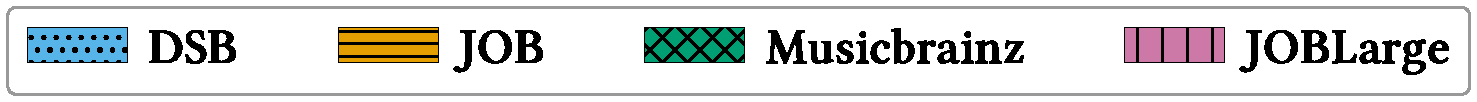
\includegraphics[width=0.55\linewidth]{figs/exp/overall-speedup-stacked/overall-speedup-legend.pdf}
    
    \vspace{0.25\baselineskip}
    
    \begin{subfigure}[b]{0.49\linewidth}
        \centering
        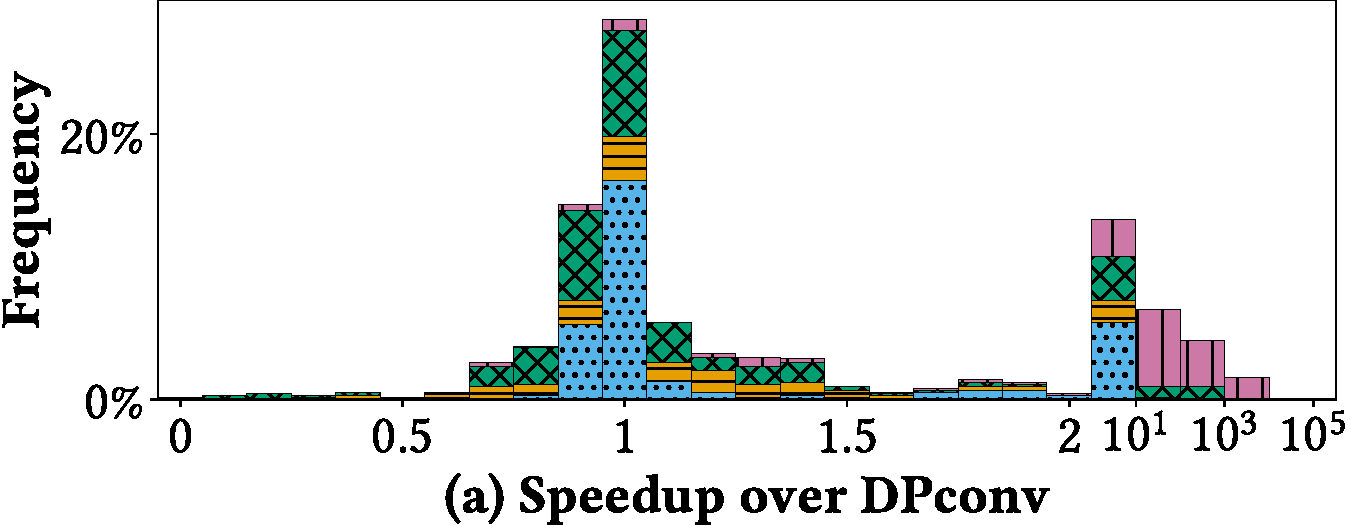
\includegraphics[width=\linewidth]{figs/exp/overall-speedup-stacked/overall-speedup-over-dpconv.pdf}
        % \caption{Over DPconv}
        \label{fig:overall-speedup-dpconv}
    \end{subfigure}
    \hfill
    \begin{subfigure}[b]{0.49\linewidth}
        \centering
        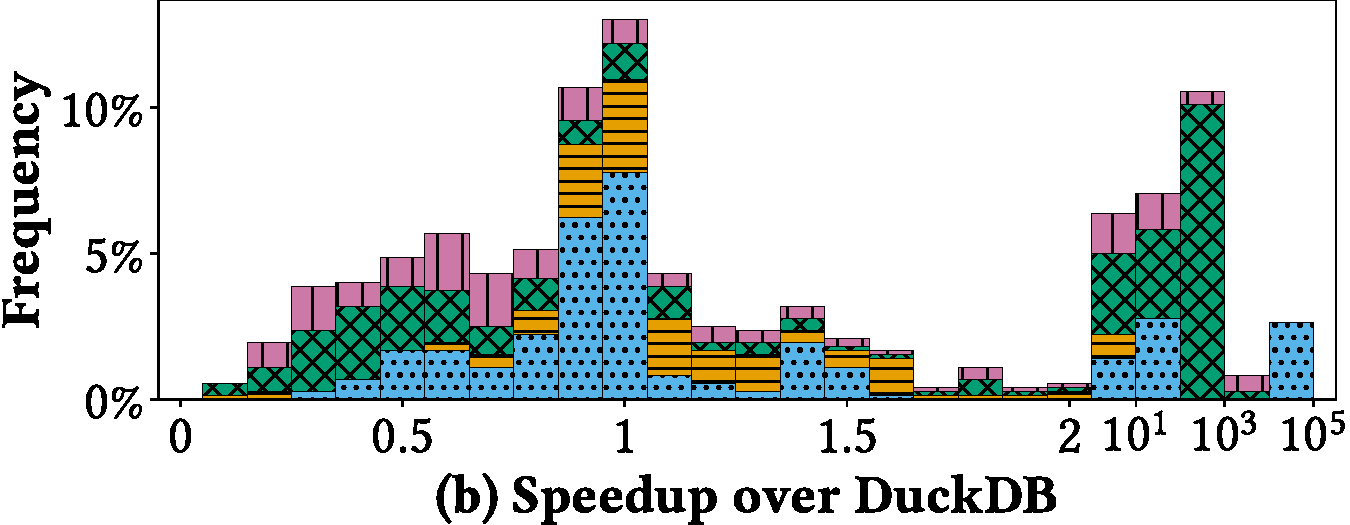
\includegraphics[width=\linewidth]{figs/exp/overall-speedup-stacked/overall-speedup-over-duckdb.pdf}
        % \caption{Over DuckDB}
        \label{fig:overall-speedup-duckdb}
    \end{subfigure}
    
    \vspace{-0.5\baselineskip}
    
    \begin{subfigure}[b]{0.49\linewidth}
        \centering
        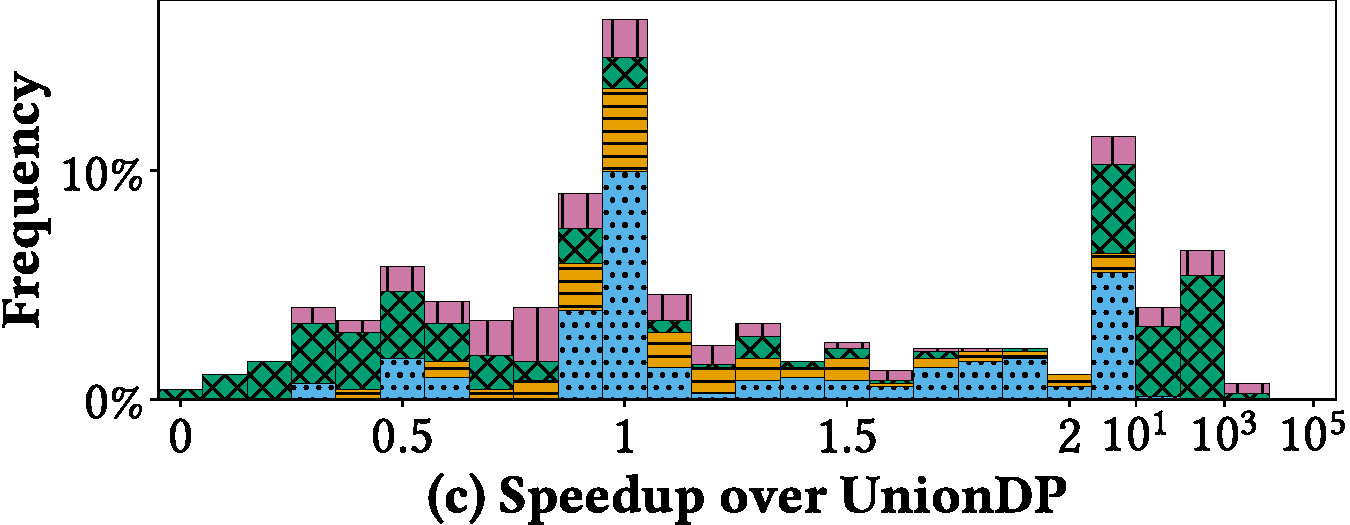
\includegraphics[width=\linewidth]{figs/exp/overall-speedup-stacked/overall-speedup-over-uniondp.pdf}
        % \caption{Over UnionDP}
        \label{fig:overall-speedup-uniondp}
    \end{subfigure}
    \hfill
    \begin{subfigure}[b]{0.49\linewidth}
        \centering
        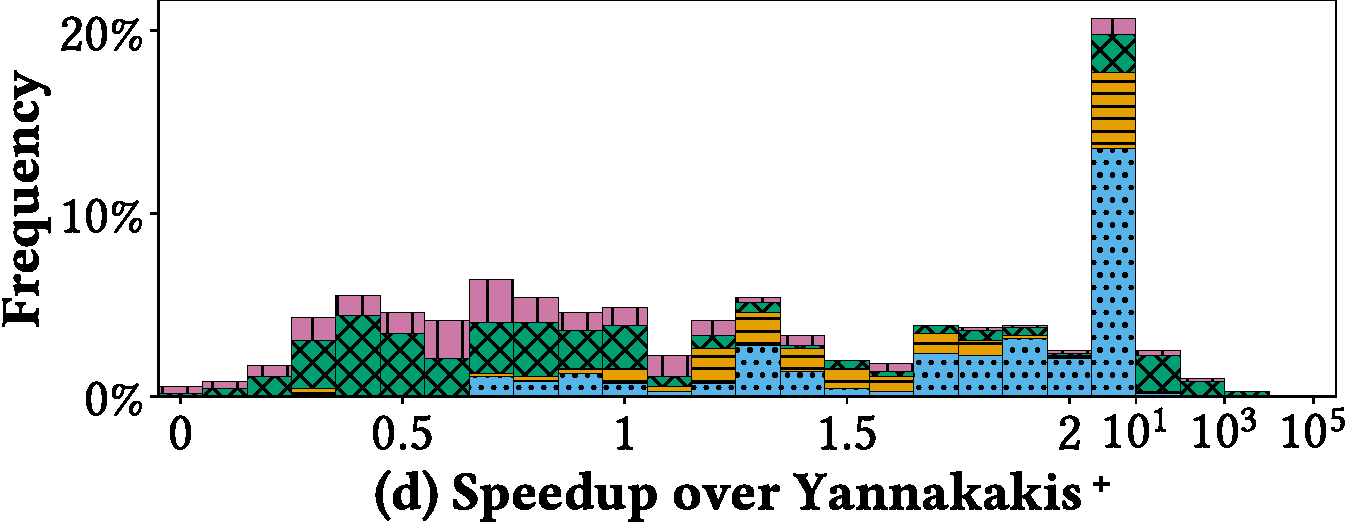
\includegraphics[width=\linewidth]{figs/exp/overall-speedup-stacked/overall-speedup-over-yanplus.pdf}
        % \caption{Over Yannakakis$^+$}
        \label{fig:overall-speedup-yanplus}
    \end{subfigure}

    \vspace{-0.5\baselineskip}

    \begin{subfigure}[b]{0.49\linewidth}
        \centering
        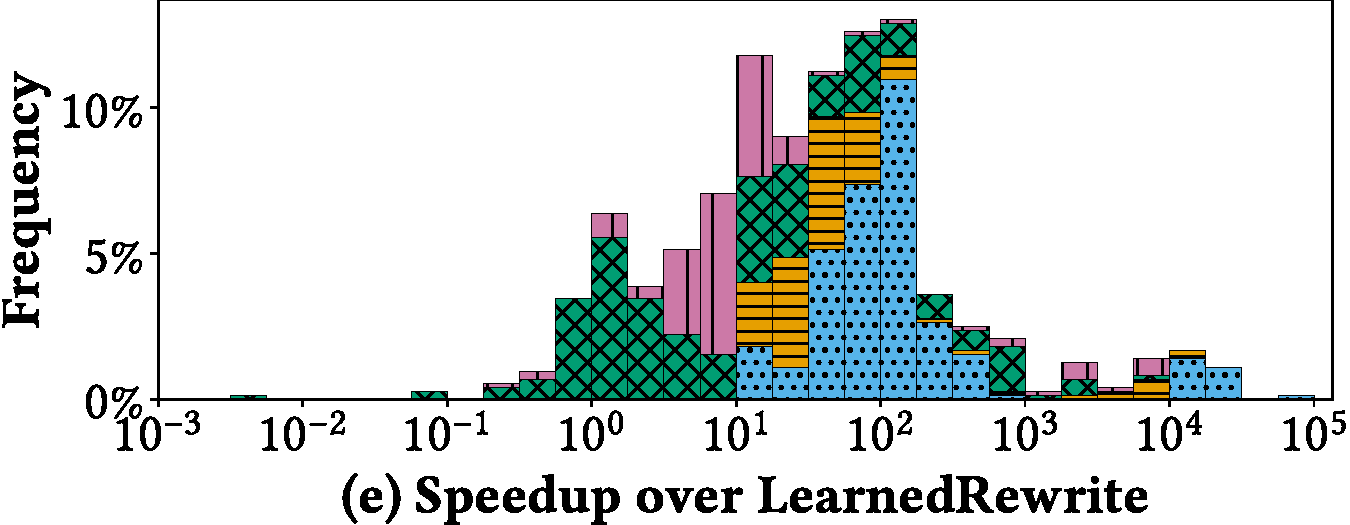
\includegraphics[width=\linewidth]{figs/exp/overall-speedup-stacked/overall-speedup-over-learned-rewrite.pdf}
        % \caption{Over Learned Rewrite}
        \label{fig:overall-speedup-learned-rewrite}
    \end{subfigure}
    \hfill
    \begin{subfigure}[b]{0.49\linewidth}
        \centering
        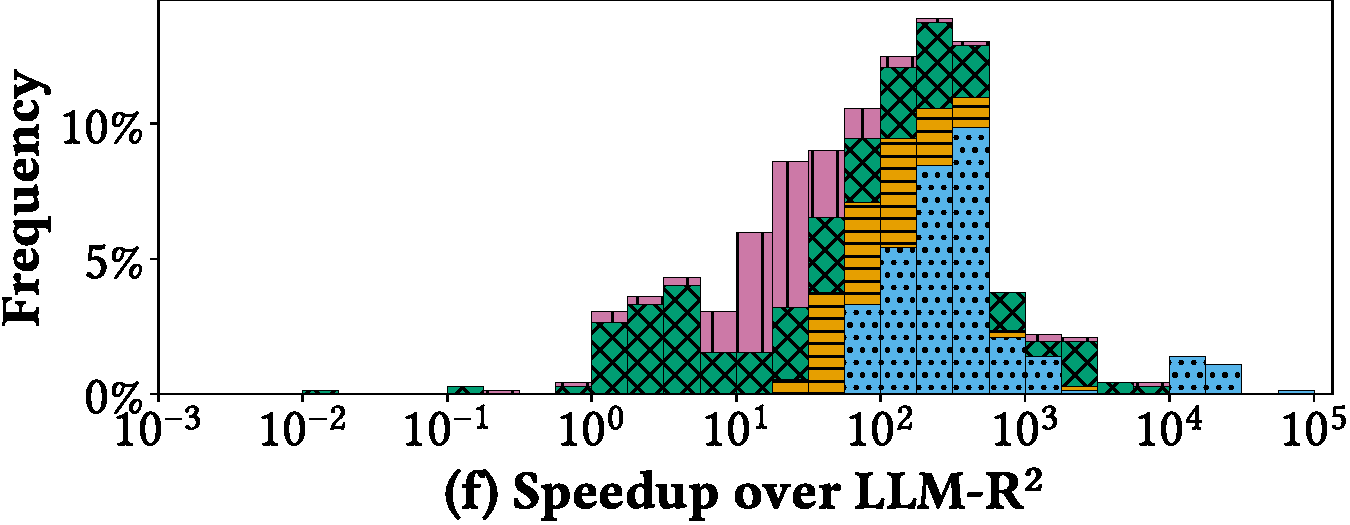
\includegraphics[width=\linewidth]{figs/exp/overall-speedup-stacked/overall-speedup-over-llm-r2.pdf}
        % \caption{Over LLM-R$^2$}
        \label{fig:overall-speedup-llm-r2}
    \end{subfigure}
    
    \vspace{-1.5\baselineskip}
    
    \caption{Histograms of overall speedups of using \sys{} over using other methods}
    \label{fig:overall-speedup-histogram}
\end{figure}
\begin{figure}
    
\includegraphics[width=0.55\linewidth]{figs/exp/scatter-all-benchmarks/scatter-legend.pdf}
    
    \vspace{0.5\baselineskip}
    
    \begin{subfigure}[b]{0.28\linewidth}
        \centering
        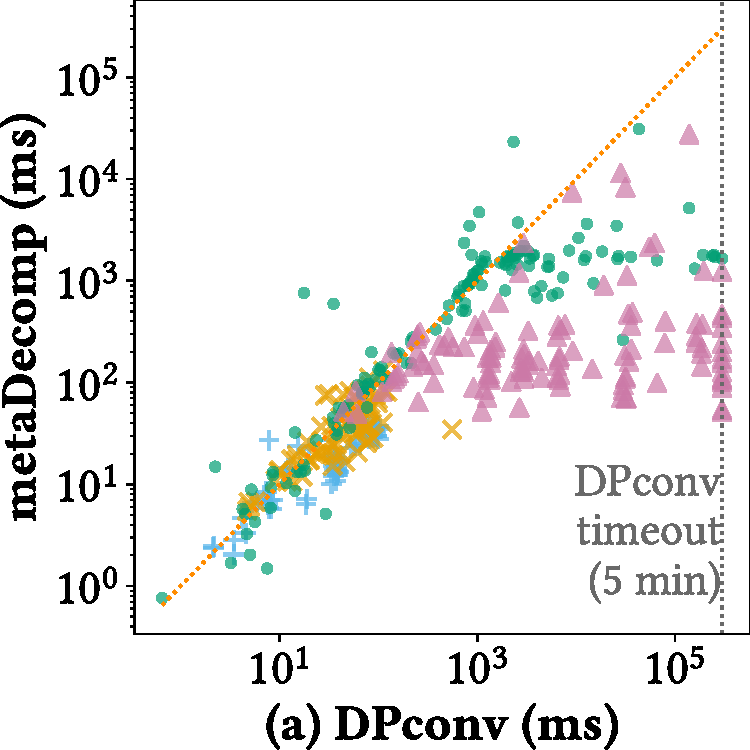
\includegraphics[width=\linewidth]{figs/exp/scatter-all-benchmarks/scatter-meta-dpconv.pdf}
        \label{fig:overall-scatter-dpconv}
    \end{subfigure}
    \hfill
    \begin{subfigure}[b]{0.28\linewidth}
        \centering
        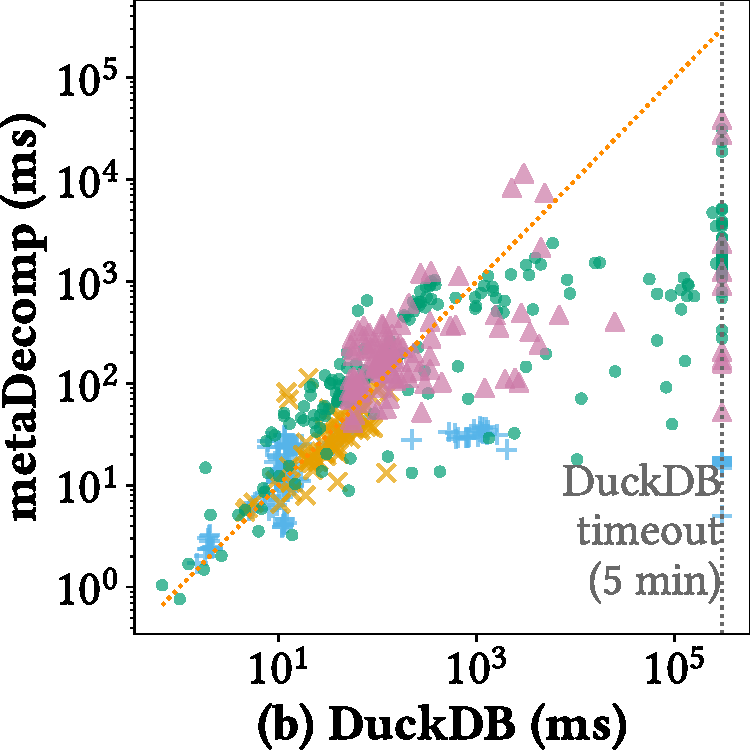
\includegraphics[width=\linewidth]{figs/exp/scatter-all-benchmarks/scatter-meta-duckdb.pdf}
        \label{fig:overall-scatter-duckdb}
    \end{subfigure}
    \hfill
    \begin{subfigure}[b]{0.28\linewidth}
        \centering
        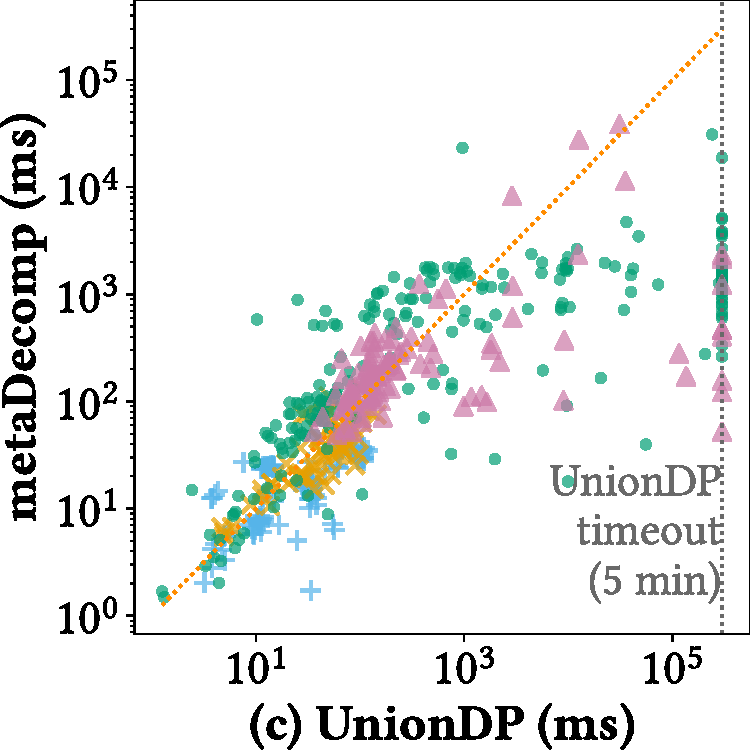
\includegraphics[width=\linewidth]{figs/exp/scatter-all-benchmarks/scatter-meta-uniondp.pdf}
        \label{fig:overall-scatter-uniondp}
    \end{subfigure}
    
    \vspace{-0.5\baselineskip}
    
    \begin{subfigure}[b]{0.28\linewidth}
        \centering
        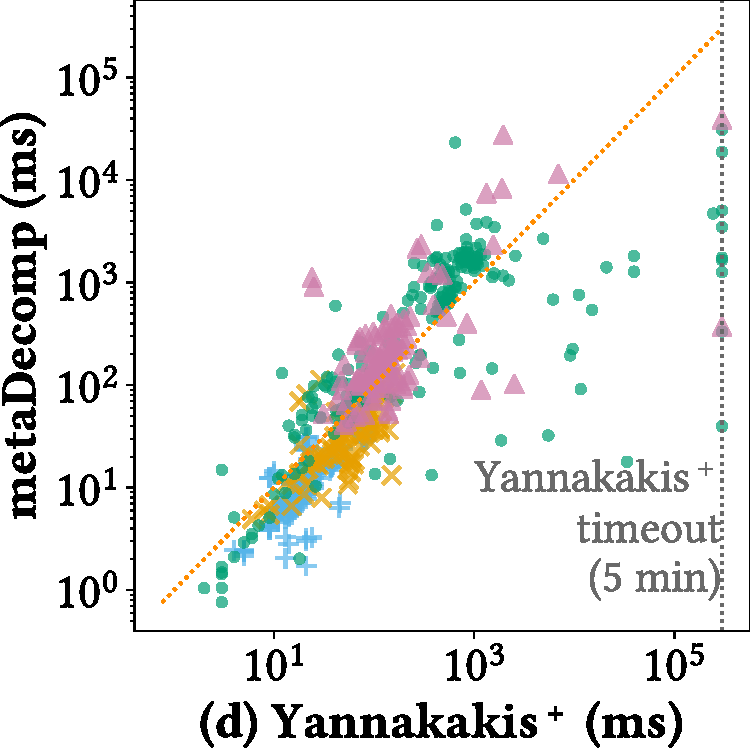
\includegraphics[width=\linewidth]{figs/exp/scatter-all-benchmarks/scatter-meta-yanplus.pdf}
        \label{fig:overall-scatter-yanplus}
    \end{subfigure}
    \hfill
    \begin{subfigure}[b]{0.28\linewidth}
        \centering
        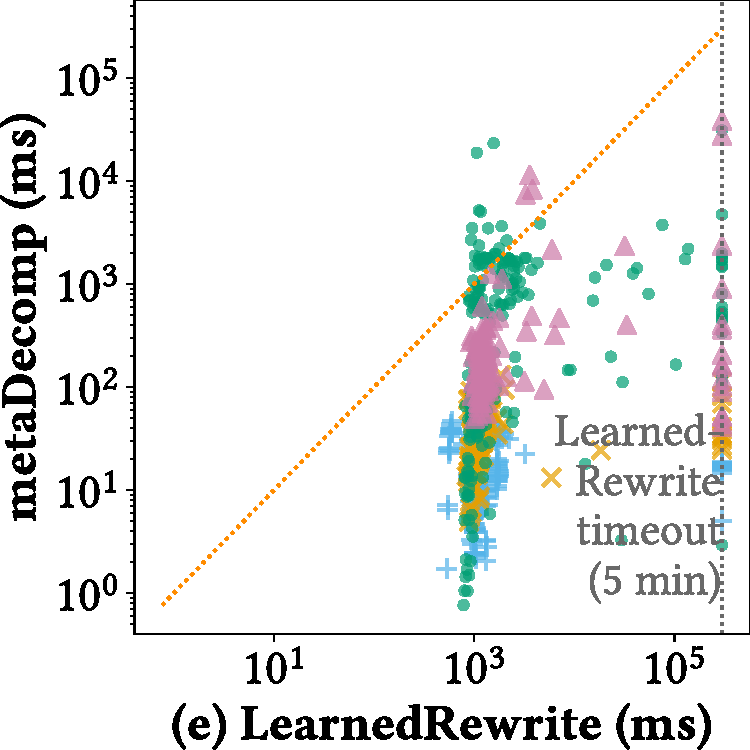
\includegraphics[width=\linewidth]{figs/exp/scatter-all-benchmarks/scatter-meta-learned-rewrite.pdf}
        \label{fig:overall-scatter-learned-rewrite}
    \end{subfigure}
    \hfill
    \begin{subfigure}[b]{0.28\linewidth}
        \centering
        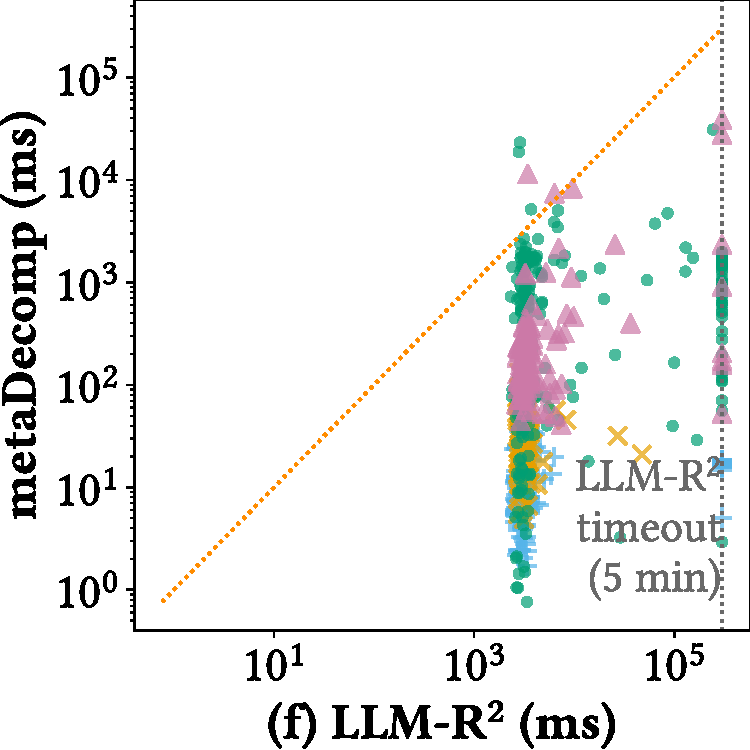
\includegraphics[width=\linewidth]{figs/exp/scatter-all-benchmarks/scatter-meta-llm-r2.pdf}
        \label{fig:overall-scatter-llm-r2}
    \end{subfigure}
    
    \vspace{-1.5\baselineskip}
    \caption{Scatter plots of overall evaluation time using metaDecomp versus using other methods. Queries for which the difference is less than 10\% are omitted in the figures.}
    \label{fig:overall-scatter}
    \vspace{0.5\baselineskip}
\end{figure}
}

Taking both optimization and execution time into account, we observe in \cref{tab:stats-new}, \cref{fig:overall-speedup-histogram}, and \cref{fig:overall-scatter} that \sys{} shows a clear advantage overall. This is especially the case for queries that are complex, as shown by the 95th and 99th percentiles in \cref{tab:stats-new}, and in the points towards the right in the scatter plots in \cref{fig:overall-scatter}. 
For DuckDB, UnionDP, Yannakakis$^+$, LearnedRewrite, and LLM-R$^2$, although their optimization is fast, they are also very likely to generate plans that are significantly worse than the optimal width-1 query plans, especially for larger queries.
In addition, for Yannakakis$^+$, there is an overhead in the reduction phase, which may be costly for certain queries.
For DPconv, the main disadvantage is the exponential optimization time, which becomes the dominant factor in the overall evaluation time for large queries.
The overall results demonstrate that finding and executing width-1 plans with \sys{} is indeed highly efficient in practice.
More detailed, separate figures for individual benchmarks can be found in the \arxivorappendix.

\subsubsection{\ref{RQ3} Sensitivity to cardinality misestimation}
Recent research has shown that structure-based query optimization tends to be more robust even in the presence of errors in cardinality estimation~\cite{wang_yannakakis_2025,DiamondJoin2024,RPT2025}.
This is also the case for \sys{}.
To illustrate, we compare \sys{} with DPconv and UnionDP, which use the exact same cost model. We run them on DSB and JOB queries with (1) exact and (2) misestimated cardinalities.
The misestimated cardinalities are generated by adding a multiplicative noise to the exact cardinalities using a log-normal distribution. Specifically, for each exact cardinality $C$, we generate a perturbed estimate $\hat{C} = C \cdot e^\epsilon$, where $\epsilon \sim \mathcal{N}(0, \sigma^2)$, i.e., following a normal (Gaussian) distribution, with standard deviation $\sigma$ set to $10$.
From the results in \cref{tab:misestimation}, \sys{} still has excellent performance despite such errors in cardinality estimation.
The advantage is particularly pronounced at the 99th percentile of the JOB benchmark, where DPconv and UnionDP, which rely solely on cardinality values, are significantly misled by the highly inaccurate estimation.


\begin{table}
    % \centering
    \begin{footnotesize}
        % \renewcommand{\arraystretch}{1.1}
        % \setlength\tabcolsep{1pt}

\begin{tabular}{cc|cccc|cccc}
    \hline
    \multicolumn{2}{r|}{\textbf{Benchmark $\rightarrow$}}
        & \multicolumn{4}{c|}{\textbf{DSB}} & \multicolumn{4}{c}{\textbf{JOB}} \\
    \textbf{Method $\downarrow$} & \textbf{Cardinality $\downarrow$}
        & Mean & Median & 95th & 99th & Mean & Median & 95th & 99th \\
    \hline
    \multirow{2}{*}{\sys{}}
        & Exact & 0.01 s & 0.01 s & 0.04 s & 0.04 s & 0.04 s & 0.03 s & 0.08 s & 0.11 s \\
        & Misestimated & 0.02 s & 0.01 s & 0.06 s & 0.12 s & 0.05 s & 0.04 s & 0.11 s & 0.15 s \\
    \hline
    \multirow{2}{*}{DPconv}
        & Exact & 0.02 s & 0.01 s & 0.09 s & 0.10 s & 0.04 s & 0.04 s & 0.09 s & 0.11 s \\
        & Misestimated & 0.03 s & 0.01 s & 0.11 s & 0.14 s & 0.46 s & 0.05 s & 0.23 s & 2.07 s \\
    \hline
    \multirow{2}{*}{UnionDP}
        & Exact & 0.03 s & 0.01 s & 0.10 s & 0.11 s & 0.05 s & 0.04 s & 0.10 s & 0.12 s \\
        & Misestimated & 0.03 s & 0.01 s & 0.11 s & 0.14 s & 0.48 s & 0.05 s & 0.22 s & 1.86 s \\
    \hline
\end{tabular}

    \end{footnotesize}
    % \vspace{-0.2em}
    \caption{Query execution time when optimized with exact vs misestimated cardinalities}
    % \vspace{-1.4em}
    \label{tab:misestimation}
\end{table}

\subsubsection{\ref{RQ4} Meta-decompositions applied to other structure-based optimization techniques}
\begin{figure}
    
\includegraphics[width=0.37\linewidth]{figs/exp/enum-time/enum-time-legend.pdf}
    
    \vspace{0.25\baselineskip}
    
    \begin{subfigure}[b]{0.24\textwidth}
        \centering
        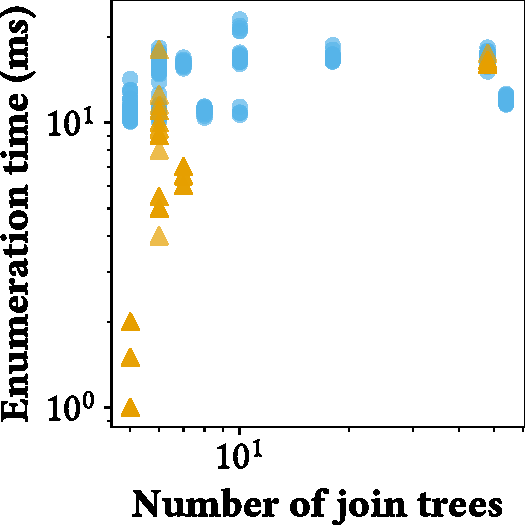
\includegraphics[width=\linewidth]{figs/exp/enum-time/enum-time-dsb.pdf}
        \caption{DSB}
        \label{fig:enum-dsb}
    \end{subfigure}
    \hfill
    \begin{subfigure}[b]{0.24\textwidth}
        \centering
        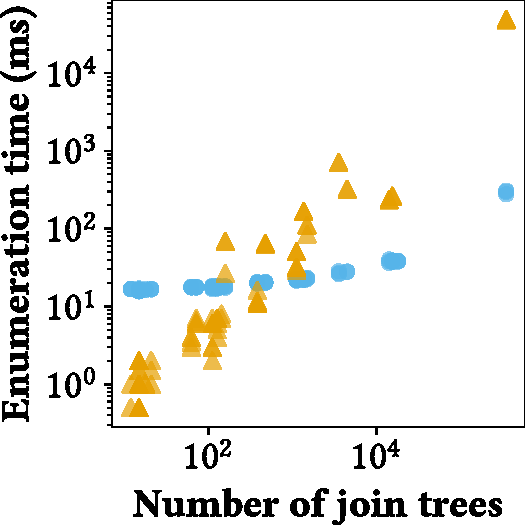
\includegraphics[width=\linewidth]{figs/exp/enum-time/enum-time-job-original.pdf}
        \caption{JOB}
        \label{fig:enum-job-original}
    \end{subfigure}
    \hfill
    \begin{subfigure}[b]{0.24\textwidth}
        \centering
        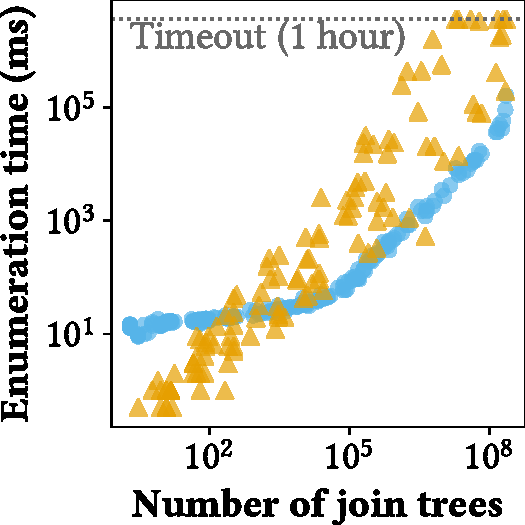
\includegraphics[width=\linewidth]{figs/exp/enum-time/enum-time-musicbrainz.pdf}
        \caption{Musicbrainz}
        \label{fig:enum-musicbrainz}
    \end{subfigure}
    \hfill
    \begin{subfigure}[b]{0.24\textwidth}
        \centering
        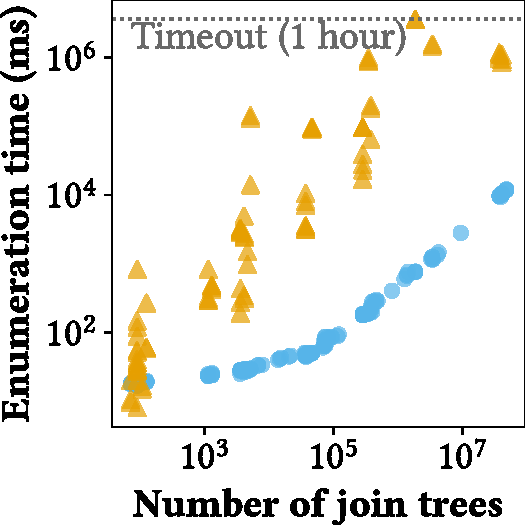
\includegraphics[width=\linewidth]{figs/exp/enum-time/enum-time-job-large.pdf}
        \caption{JOBLarge}
        \label{fig:enum-job-large}
    \end{subfigure}
    \vspace{-0.5\baselineskip}
    \caption{Scatter plots of join tree enumeration time using \sys{} versus using na\"ive GYO reduction}
    \label{fig:enum-time}
\end{figure}
Finally, we demonstrate how meta-decompositions can help other recently developed structure-based optimization techniques.
A crucial step in those techniques is selecting a good join tree, as it can significantly influence the structures and, consequently, the costs of the generated query plans.

Thus, we first evaluate \sys{}'s efficiency in \emph{enumerating join trees}, compared to the standard GYO reduction–based approach from \cite{dai_sparksql_2023}. 
As shown in \cref{fig:enum-time}, \sys{} shows up to \emph{four orders of magnitude of speedups} over the traditional approach. In particular, for many highly complex queries in the Musicbrainz and JOBLarge benchmarks with more than $10^7$ join trees, the traditional approach already takes over $1$ hour, whereas \sys{} can complete the enumeration in $2$ seconds to $1$ minute.  

A more effective approach is to apply cost-based optimization directly on meta-decompositions, as has already been done in \sys{}, since this eliminates the need to enumerate exponentially large numbers of join trees. Therefore, in our second experiment, we use Yannakakis$^+$~\cite{wang_yannakakis_2025} to rewrite queries based on join trees selected by \sys{} that induce the optimal width-1 query plans. \emph{This modification achieves an average speedup of {\rm 1.11x} on JOB queries.} This demonstrates that structure-based evaluation algorithms, such as Yannakakis$^+$, can benefit significantly from our efficient cost-based optimization framework.
